\section{Arquitectura de un Observatorio Virtual}

El VO's es un framework que ayuda a resolver distintos
problemas que enfrenta la comunidad astronómica a lo largo del mundo.  Uno de
los problemas está relacionado al acceso a los datos, por lo que en IVOA
diseñaron tecnologías y estándares formalmente definidos, que permitan el de
acceso unificado y transparente a distintos servidores con datos astronómicos.

El beneficio que conlleva es considerable, ya que estos
estándares, protocolos, tecnologías y arquitectura, ayudan a la comunidad al
proceso de creación de servicios, portales web, aplicaciones de escritorio,
etc. Todo visto del punto de vista de ingeniería de software.

\subsection{Arquitectura VO por Nivel}
%\todo{Las figuras se ven super mal en chico, quizás podrías ponerlas a doble
%columna}

IVOA dentro de sus documentos presenta distintos niveles de arquitectura
\cite{ivoa_arch}, con el objetivo de ir aclarando incrementalmente las
funcionalidades (basadas en necesidades) que requiere un VO.

\textbf{Arquitectura Nivel 0} %~\ref{fig:nivel0}\\


La arquitectura más básica que aclara el concepto de VO, se compone por 3
capas:

\begin{enumerate}
    \item Capa de recursos:
          compilado de datos astronómicos provenientes de distintos instrumentos.
    \item Capa de usuarios:
          investigadores que buscan consumir datos.
    \item Capa intermedia:
          es la capa que permite conectar las dos
          capas anteriores de manera transparente para los investigadores.
          Esta interacción se puede llevar a cabo buscando u obteniendo datos.
\end{enumerate}

\begin{figure*}[h!t]
    \centering
    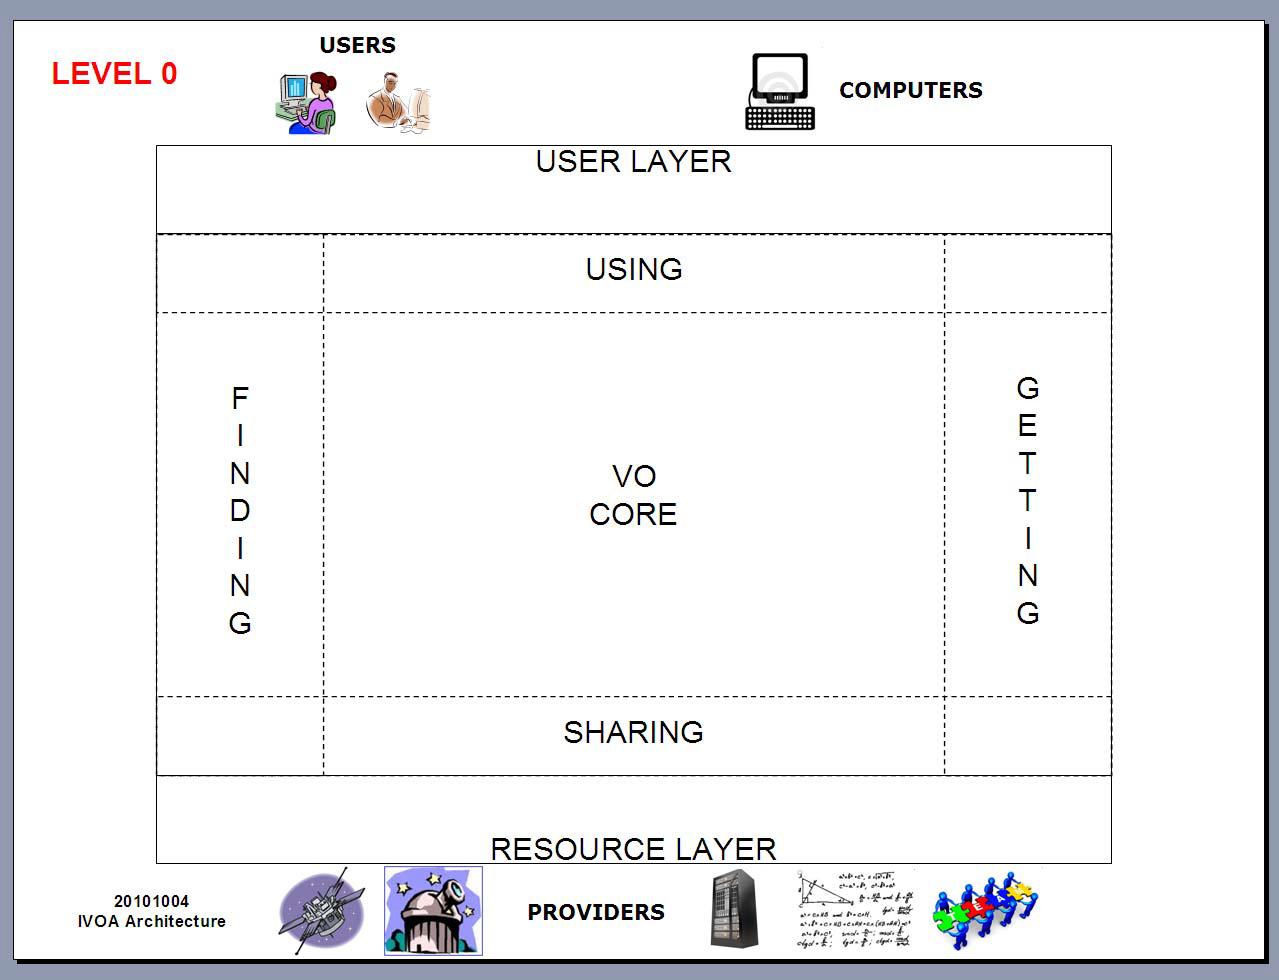
\includegraphics[width=0.7\textwidth]{img/arquitectura_0.png}
    \caption{Arquitectura Nivel 0}
    \label{fig:nivel0}
\end{figure*}

\textbf{Arquitectura Nivel 1}%~\ref{fig:nivel1}


La arquitectura nivel 1 mantiene la misma cantidad de capa pero se especifica:
\begin{enumerate}
    \item Capa de recursos:
          está compuesto de colección de datos y provenientes de distintos
          servidores.
    \item Capa de usuarios:
          un consumidor puede querer acceder a los datos desde un navegador,
          escritorio, o mediante un script.
    \item Capa intermedia:
          crea un framework para compartir los datos, compuesto por VOQL,
          Data Models, Semantics, Formats.
\end{enumerate}

\begin{figure*}[h!t]
    \centering
    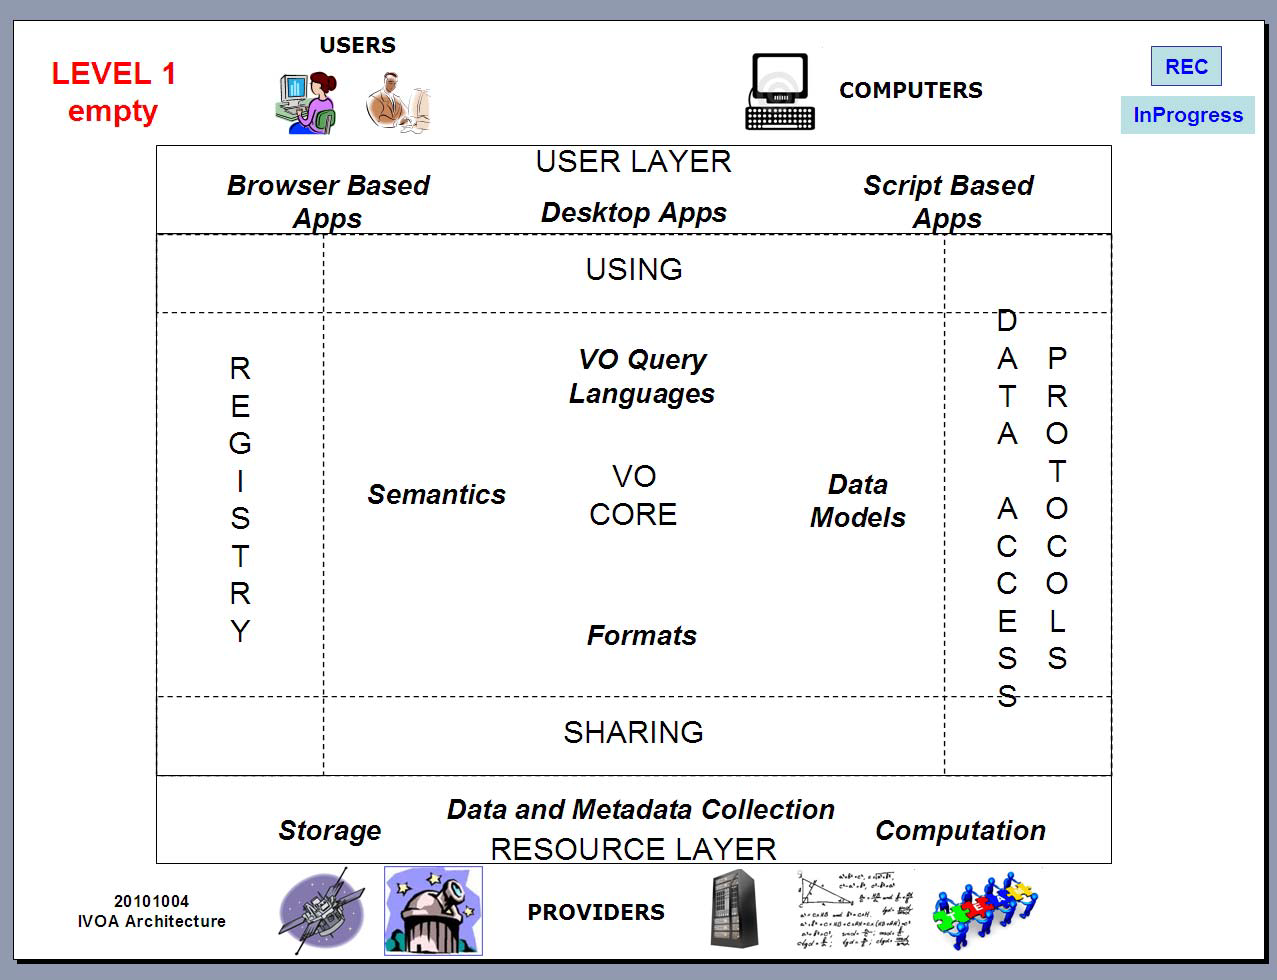
\includegraphics[width=0.7\textwidth]{img/arquitectura_1.png}
    \caption{Arquitectura Nivel 1}
    \label{fig:nivel1}
\end{figure*}

\textbf{Arquitectura Nivel 2}%~\ref{fig:nivel2}


La arquitectura nivel 2 es lo que se entiende por un VO regido por estándares
y protocoloes de IVOA.
La idea de esta figura es seccionar cada estándar relacionándolo específicamente
a la capa a la cual pertenece.

\begin{figure*}[h!t]
    \centering
    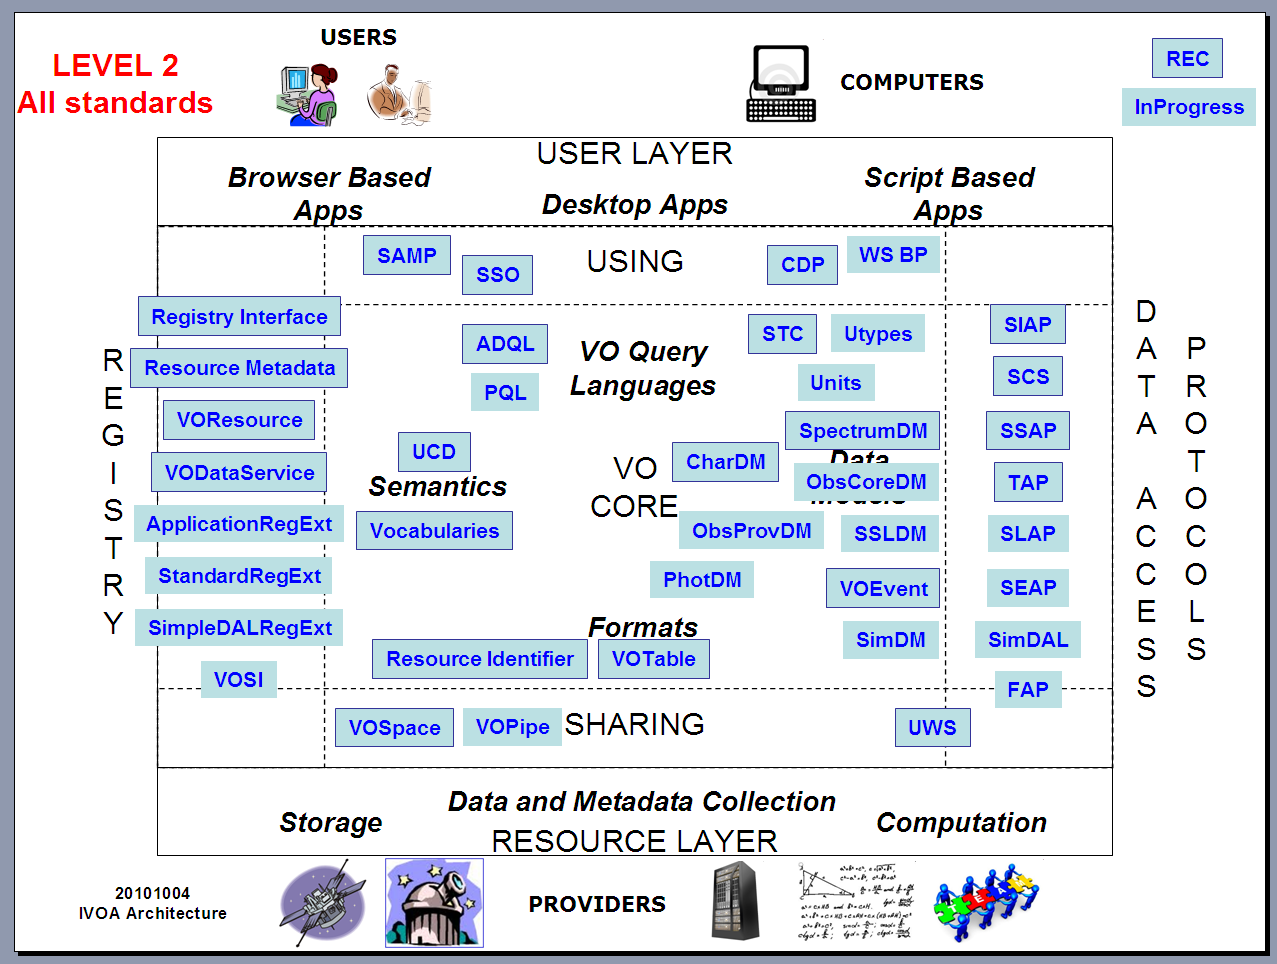
\includegraphics[width=0.7\textwidth]{img/arquitectura_2.png}
    \caption{Arquitectura Nivel 2}
    \label{fig:nivel2}
\end{figure*}
